\section{Server}
Il package \texttt{Server} contiene le classi necessarie per 
la gestione del server, che si occupa di gestire le richieste 
dai client interfacciandosi con il database.

\subsection{Main}
La classe \texttt{ServerTK} contiene il metodo \texttt{main} 
che avvia il server e gestisce le connessioni dei client.
All'avvio del server vengono richieste le credenziali per stabilire 
una connessione con il database e, una volta creata, viene generato un 
registro RMI per poter esporre i servizi offerti dal server.
\begin{figure}[H]
  \centering
  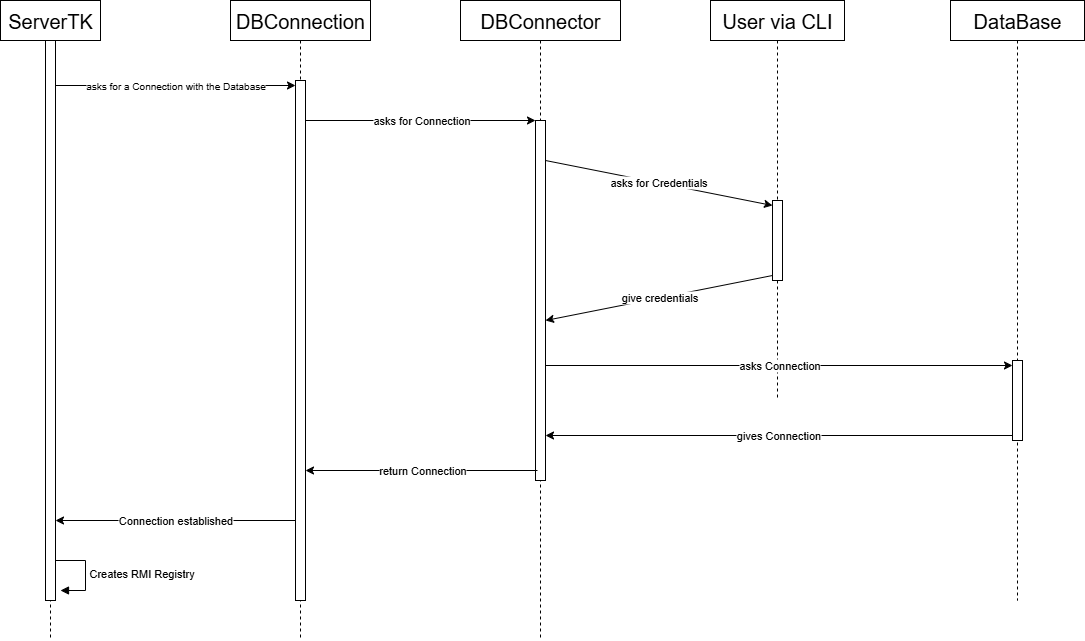
\includegraphics[width=\textwidth]{images/UML-interaction-server.png}
  \caption{Interaction Diagram - Server Start-Up}
  \label{fig:interaction-diagram-server}
\end{figure}

\subsubsection{DBConnection}
La classe \texttt{DBConnection} si occupa di stabilire
una singola connessione col Database e rendenderla disponibile 
alle altre classi del server tramite il design pattern \textit{Singleton}.
Per ottenere la connessione al database, viene utilizzata la classe 
\textit{DBConnector} che si occupa di richiedere le credenziali 
all'utente e tentare la connesione.

\subsection{Data Access Object}
Il package \texttt{dao} contiene le classi che implementano 
il pattern Data Access Object (DAO) per l'interazione
con il database isolando la logica di persistenza.
Queste classi sono responsabili dell'interazione 
del database con l'applicazione.
Le classi implementate sono le seguenti:
\begin{itemize}
    \item \texttt{UserDAO}: gestisce le operazioni relative alla tabella \textit{\hyperref[sec:users]{users}}
    \item \texttt{RestaurantDAO}: gestisce le operazioni relative alla tabella \textit{\hyperref[sec:restaurants]{restaurants}}
    \item \texttt{AddressDAO}: gestisce le operazioni relative alla tabella \textit{\hyperref[sec:addresses]{addresses}}
    \item \texttt{ReviewDAO}: gestisce le operazioni relative alla tabella \textit{\hyperref[sec:reviews]{reviews}}
\end{itemize}
Queste classi semplificano la gestione dei dati permettendo 
di interfacciarsi col database senza preoccuparsi delle specifiche
implementative dello stesso. 
In queste classi sono implementate le queries per l'inserimento, 
la modifica e l'eliminazione dei dati e gestiscono in autonomia 
le eccezioni che possono verificarsi durante l'interazione
con il database.
\paragraph{PreparedStatement}
Tutte le queries sono implementate utilizzando la classe
\texttt{PreparedStatement} per garantire la sicurezza
dell'applicazione, prevenire attacchi di tipo SQL Injection, 
migliorare le performance attraverso caching delle queries compilate
e semplificarne la scrittura.
\paragraph{Favorites}
Notare che non è stato implementato un DAO per la tabella \textit{\hyperref[sec:favorites]{favorites}}
poiché essendo un'entità di relazione tra \textit{users} e \textit{restaurants} 
si è ritenuto sufficiente gestirla tramite \texttt{RestaurantDAO}; 
le queries per la gestione dei preferiti sono dunque implementate
all'interno di quest'ultima classe.
\paragraph{Formula di Haversine}
Per il calcolo della distanza tra due punti sulla superficie terrestre
è stata implementata la \textit{Formula di Haversine}.
\begin{minted}{sql}
(
  6371 * ACOS(
    COS(radians(?)) * COS(radians(latitude)) * 
    COS(radians(longitude) - RADIANS(?)) + 
    SIN(radians(?)) * SIN(RADIANS(latitude))
  )
) AS distance 
\end{minted}

\subsection{Server Services}
Il package \texttt{server\_services} contiene le classi che implementano
le interfacce definite nel package \texttt{common}.
Queste classi vengono esposte dal database in un \texttt{Registry}
e rese accessibili ai client tramite JavaRMI.
I metodi delle classi garantiscono una corretta gestione della 
concorrenza e utilizzano le classi DAO per interagire con il database.
Le classi implementate sono le seguenti:
\begin{itemize}
    \item \texttt{RestaurantServiceImpl.java} implementa \texttt{\hyperref[sec:restaurantservice]{RestaurantService}}
    \item \texttt{ReviewServiceImpl.java} implementa \texttt{\hyperref[sec:reviewservice]{ReviewService}}
    \item \texttt{UserServiceImpl.java} implementa \texttt{\hyperref[sec:userservice]{UserService}}
\end{itemize}
